\documentclass[12pt]{article}
\usepackage[margin=1in]{geometry}
\usepackage{mathtools}
\usepackage{xcolor}
\usepackage{hyperref}
\hypersetup{
    colorlinks=true,
    linkcolor=blue,   
    urlcolor=blue,
}
\usepackage{setspace}
\usepackage[utf8]{inputenc}
\doublespacing
\usepackage{hyperref}

\usepackage{siunitx}
\DeclareSIUnit \parsec {pc}
\sisetup{separate-uncertainty=true, multi-part-units=single, parse-numbers = false}

\BeforeBeginEnvironment{align}{\begin{singlespace}}
\AfterEndEnvironment{align}{\end{singlespace}\noindent\ignorespaces}

\renewcommand{\l}{\ell}
\newcommand{\ex}[1]{\left\langle#1\right\rangle}
\renewcommand{\th}[1]{\frac{1}{#1}}

\newcommand{\units}{\kilo\meter\per\second\per\mega\parsec}
\newcommand{\hnaught}[1]{\SI{#1}{\units}}
\newcommand{\note}[1]{\textcolor{red}{#1}}
\newcommand{\outline}[1]{\textcolor{teal}{#1}}
\renewcommand{\L}{$\Lambda$}
\newcommand{\eff}{\text{eff}}
\newcommand{\val}[1]{\cite{DiValentino2021} Sec.~#1}
\newcommand{\Planck}[1]{\textit{Planck}}
\newcommand{\nn}{\nonumber\\}
\newcommand{\DE}{\text{DE}}

\title{Tension in the Hubble Constant}
\author{Charles Stahl}
\date{\today}

\begin{document}

\begin{singlespace}
\maketitle

\begin{abstract}
\normalsize
The Hubble constant $H_0$ measures the rate at which distant objects are receding away from us, as a function of their distance. In effect, it measures how fast our Universe is expanding. Although $H_0$ can be measured in our local region, it can also be inferred using the Cosmic Microwave Background (CMB) and the current standard model of cosmology, the Lambda-Cold Dark Matter (\L CDM) model. Together, the measurement and the inference can provide a check of the validity of the model. Recently, errors bars on both methods of arriving at $H_0$ have grown small enough to put them in tension. Here we review the tension and some attempts at relieving it.
\end{abstract}
\end{singlespace}

\section{Introduction and History} \label{sec:int}

When Einstein published the general theory of relativity in 1916~\cite{Einstein1916}, it did not take long for the scientific community to realize it implied the Universe was evolving. The next year, he showed that the Universe could be static if the equations for GR included an extra constant, now called the cosmological constant $\Lambda$~\cite{Einstein1917}.

Throughout the 1920s scientists such as Friedmann and Lema\^{i}tre continued to explore the possibility of an expanding universe~\cite{Friedman1922, Lemaitre1927}. In 1929 Edwin Hubble published his observation that the Universe was in fact expanding~\cite{Hubble1929}, leading Einstein to call the introduction of the cosmological constant a blunder.\footnote{There is some controversy over George Gamow's claim that Einstein called it his ``greatest blunder".} Einstein would never again use the cosmological constant in a published paper.

Hubble's measurements showed a linear relationship between an object's distance from Earth and its velocity, which implied that space itself is expanding. Although Hubble's data were far from perfect, observations have improved in the decades since. A comparison can be seen in Fig.~\ref{fig:Hubble}. The slope of this graph, in units of $\hnaught{}$, is called the Hubble constant, $H_0$.

\begin{figure}
\centering
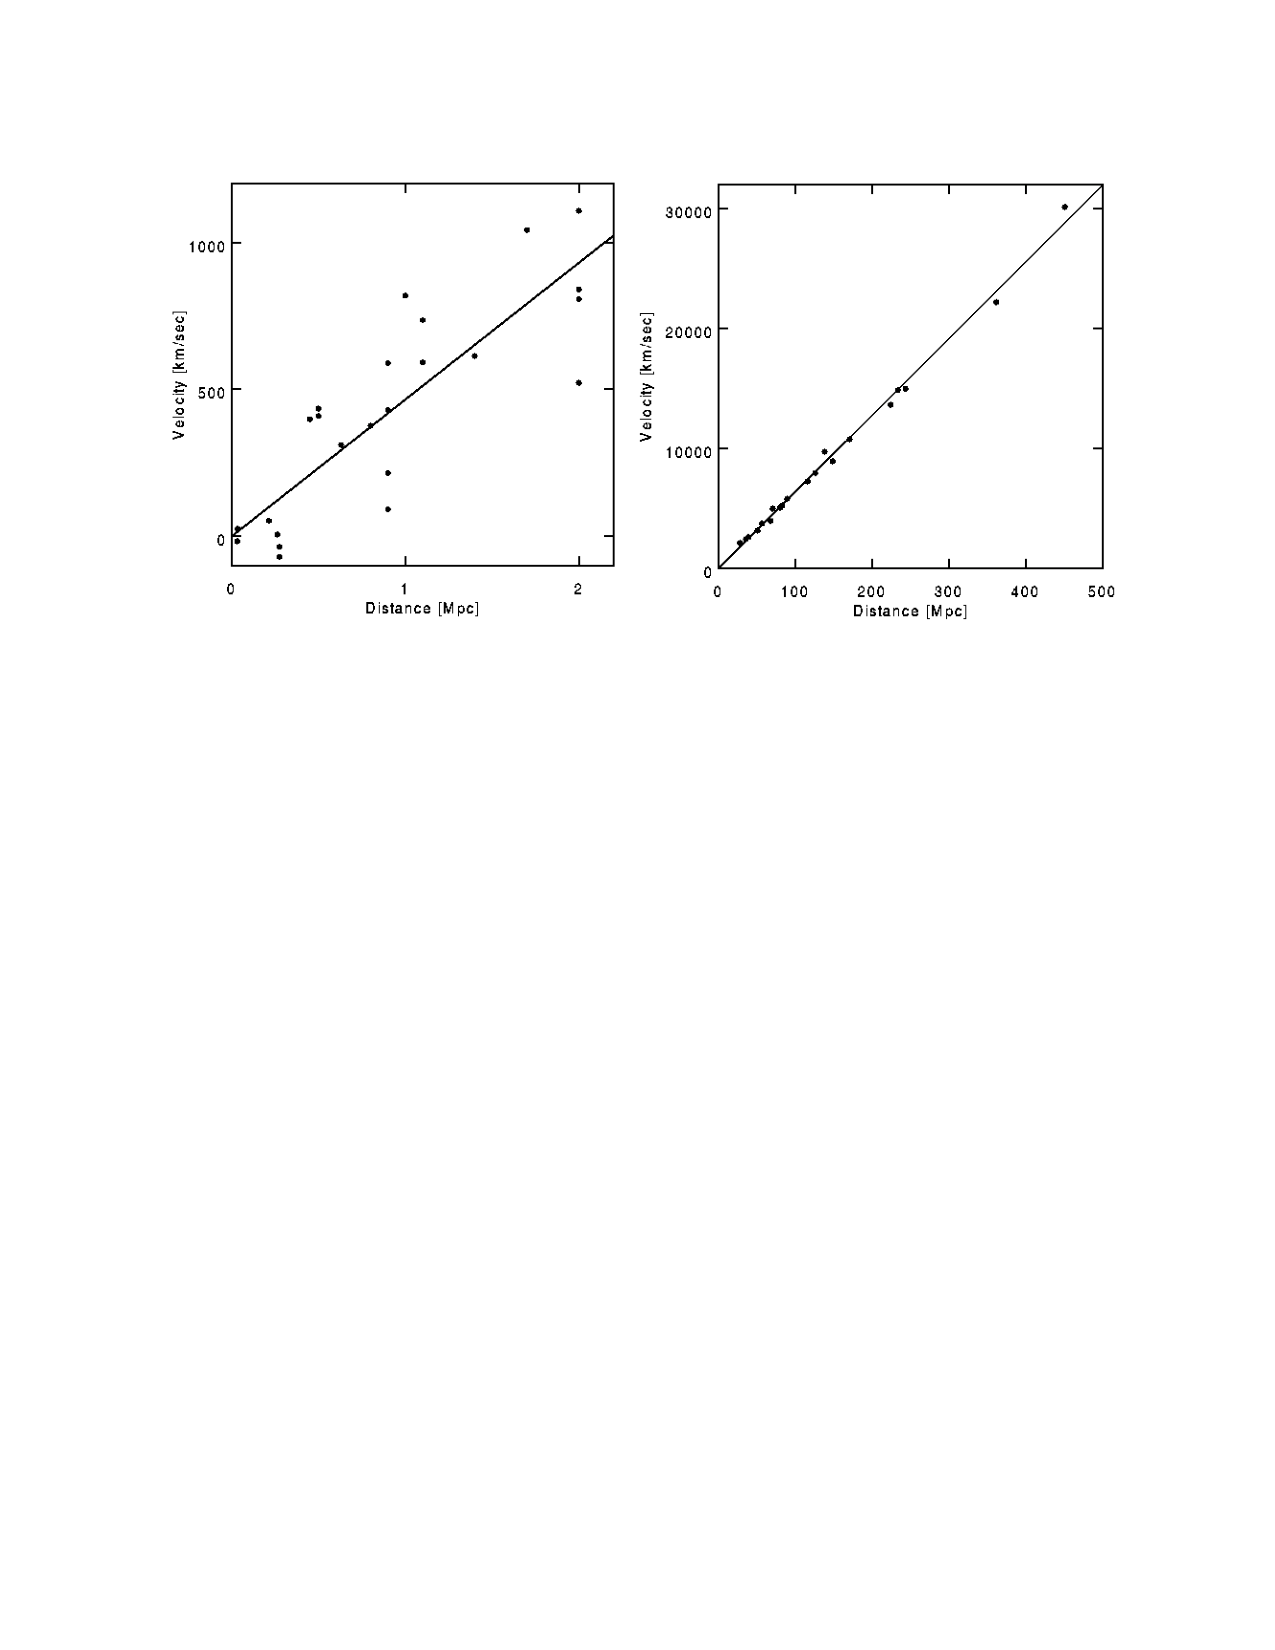
\includegraphics[]{Hubble}
\caption{Comparison of Hubble's original data with more modern observations, from Ref.~\cite{Trodden2004}. Note the much larger distance scale on the right, and the improved linear fit.}
\label{fig:Hubble}
\end{figure}

In addition, our understanding of cosmology has improved. The current standard model of cosmology is still based on the fundamental work of Friedmann and Lema\^itre, along with Robertson and Walker. Called the Lambda-cold dark matter (\L CDM) model, it describes a Universe that started with a Big Bang and evolved under general relativity with contents consisting of matter, radiation, and some from of cosmological constant \L. 

A key confirmation of the Big Bang came in 1965 when Penzias and Wilson tried to make a really good radio antenna. They kept trying to remove some background in the microwave range that was present no matter where they looked in the sky. Finally, they realized this background was actually predicted by the Big Bang model, as leftover radiation from the time of recombination.~\cite{Penzias1965}. 

Soon after the Big Bang the universe was very hot. Eventually it reached a state in which the dominant form of matter was protons and electrons. At this point, the matter and was coupled to the radiation and the temperature was high enough to keep the matter ionized. Thus, the universe was a plasma, and the plasma was opaque.
In this phase the entire universe was in thermal equilibrium. Note that this fact alone is surprising, since we know that there were points in thermal equilibrium that were outside each other's cosmic horizons. This is one of the motivations for inflation. 

Eventually (300\;000 years after the Big Bang), the Universe cooled down enough to let atoms form (recombination). At this point the matter and radiation lost contact and the photons were able to free-stream (decoupling). This moment in time is called the surface of last scattering.  The photons from last scattering are still traveling through the now-transparent Universe, and we see them as a background microwave signal coming from every direction.

Although this cosmic microwave background (CMB) is extremely uniform, it has some anisotropies. In the 1990s cosmologists figured out how to use these perturbations to confirm the \L CDM model and also make predictions. In particular, it is possible to use the CMB to predict the value of $H_0$. Initially, the value predicted from the CMB and the value measured by observations did not agree, but had large enough error bars that the two values were compatible. 

In recent years, both methods have drastically decreased their error bars without converging. The result is that today the two methods are in tension with each other with a statistical significance of $4-6\sigma$~\cite{DiValentino2021}. It is possible that one method suffers from systematic bias, but if not then the \L CDM model needs to be updated. This disagreement, called the Hubble tension, has been the topic of many recent conferences~\cite{Verde2019, DiValentino2020}.  In this paper we will describe how both methods arrive at a value for $H_0$ and summarize some possible resolutions to the tension.

The primary source for this paper will be Ref.~\cite{DiValentino2021}, which reviews various classes of resolutions to the tension. We will refer to sections in that review as (\val{1}), etc, so that the interested reader can find more detailed information. We will start, however, by reviewing some helpful background material in order to provide the reader with a more gentle introduction to the Hubble tension. Throughout, we will set $c = 1$, but convert back to useful units when reporting values for $H_0$.

\section{Background: Cosmology} \label{sec:bac}

In order to understand the tension in the Hubble constant, we will take a step back and review the history of the universe.
Our tool here will be relativistic cosmology, which describes the evolution of the universe on the largest scales. All material in this section is taken from Ref.~\cite{Trodden2004}, unless otherwise noted. We will take only the bare bones for understanding the CMB prediction of $H_0$, but the interested reader can find more detail in that reference.

The Robertson-Walker (or Friedmann-Lemaître-Robertson-Walker or FLRW) metric is the most general spacetime metric consistent with homogeneity and isotropy. It is given by
%\begin{align}
%ds^2 = -dt^2 + a^2(t)\, \left[d\rho^2 + f^2(\rho) (d\theta^2 + \sin^2 \theta\, d\phi^2)\right],
%\end{align}
%where $f(\rho)$ is either $\sin(\rho)$, $\rho$, or $\sinh(\rho)$. We can rewrite this as 
\begin{align}
ds^2 = -dt^2 + a^2(t)\left[\frac{dr^2}{1-kr^2} + r^2 (d\theta^2 + \sin^2 \theta d\phi^2)\right], \label{eqn:metric}
\end{align}
where
$k$
%\begin{align}
%k = \begin{cases}
%-1,&\qquad f(\rho) = \sinh(\rho),\\
%0,&\qquad f(\rho) = \rho,\\
%1,&\qquad f(\rho) = \sin(\rho),
%\end{cases}
%\end{align}
is the curvature index. 
%It is interesting to note that $k$ only controls the local curvature not the topology. So it is possible to have, for example, a closed universe with $k=0$, a torus. 
Our Universe is very close to flat, so we will set $k=0$ for the rest of this paper.
In these equations $t$ is called the cosmic time, which is the time measured by a comoving observer. The function $a(t)$ is called the scale factor. Moving backward in time we might find a value $t_\text{min}$ such that $a(t_\text{min})=0$. This is the Big Bang. It is convenient to define $t_\text{min} = 0$.

%From the scale factor we can define the redshift $z$. If light is emitted with wavelength $\lambda$ when the scale factor is $a$, then if it is observed when the scale factor is $a_0$ it will have wavelength $\lambda_0 = \lambda\, a_0/a$. If we place the observer at our timeslice so that $a_0=1$, then we can define the redshift
%\begin{align}
%z = \th{a}-1, \label{eqn:redshift}
%\end{align}
%so that $\Delta\lambda = z\lambda$.

From the scale factor we can define the Hubble parameter
$H = \dot{a}/a$,
where $\dot{a} = da/dt$. This value, often called the Hubble constant, is constant in space but not in time. The current value, $H_0$, is the value of $H(t)$ at our time slice. The Hubble parameter is often reported in the literature using the standard but strange units ${H = \hnaught{100\emph{h}\,}}$.

%We could replace the coordinate time $t$ with conformal time $\tau$ which obeys $dt/d\tau = a$,
%so the metric becomes
%\begin{align}
%ds^2 = a^2(\tau)\left[-d\tau^2+dr^2 + r^2 (d\theta^2 +\sin^2\theta\,d\phi^2)\right],
%\end{align}
%where we have set $k=0$. 
%Conformal time is convenient because the speed of light is 1. It will be useful to use
%\begin{align}
%dt = a\;d\tau = \frac{da}{Ha} = -\frac{a\,dz}{H}
%\end{align}
%to convert between the variables.

From Eqn.~\ref{eqn:metric} we can see that the speed of light is $1/a$.
If an emitter emits a light signal at time $t_e$ and an observer observes the signal at $t_o$, then the comoving distance between them is
\begin{align}
r_{oe} = \int_{t_e}^{t_o}\frac{dt}{a(t)}. \label{eqn:comoving}
\end{align}
Both the observer and the emitter will agree on this value. If we instead want the proper distance as measured by the observer, we get $d_o = a(t_o)r_{oe}$. The emitter measures a proper distance of $d_e = a(t_e)r_{oe}$. Since we define the scale factor such that $a(t_0)=1$ at the present time, comoving and proper distances agree for us. Eqn.~\ref{eqn:comoving} will be necessary for calculating horizons and comoving distances. For example, in a universe with a Big Bang at $t = 0$, signals can only have traveled a comoving distance of $\int_0^t\,dt'/a(t)$ by time $t$.

%For a Universe with a Big Bang at $\tau = t = 0$, we can calculate the particle horizon distance $r_{\text{ph}}(\tau) = \tau$. This measures the distance to which an observer can see. We can convert the equation to
%\begin{align}
%d_H = a(\tau)r_\text{ph} = a(\tau)\tau = a(t) \int_{0}^t\frac{dt'}{a(t')}, \label{eqn:phoriz}
%\end{align} 
%which gives the proper horizon distance $d_H$ as a function of proper time $t$. \note{Define comoving vs proper}

In addition to the kinematic variables we need some dynamical variables. Usually, we assume the universe is made a collection of perfect fluids labeled by $i$, each defined by an energy $\rho_i$, a pressure $p_i$, and an equation of state $p_i = w_i\rho_i$ (no sum). The variable $w_i$ is called the equation of state. 

Having defined our metric and some useful variables, we can use the Einstein equation of general relativity to arrive at the Friedmann equations. The first Friedmann equation is 
\begin{align}
H^2 = \left(\frac{\dot{a}}{a}\right)^2 = \frac{8\pi G}{3} \sum_i \rho_i  + \frac{\Lambda}{3}, \label{eqn:fri1}
\end{align}
which constrains the expansion of the universe given its matter content. The famous cosmological constant $\Lambda$ is just a constant of integration. It can be absorbed as a source of the equations if we let $\rho_\Lambda=\frac{\Lambda}{8\pi G}$. Under these conventions, the energy content of the universe is matter $\rho_m$ (including baryonic matter $\rho_b$ and cold dark matter $\rho_c$), radiation $\rho_r$, and dark energy $\rho_\Lambda$.

The second Friedmann equation is the evolution equation,
\begin{align}
\dot{H} + \frac{3}{2}H^2 = \frac{\ddot{a}}{a} + \frac{1}{2} \left(\frac{\dot{a}}{a}\right)^2 = -4\pi G\sum_i p_i  + \frac{\Lambda}{2}, \label{eqn:fri2}
\end{align}
where we can again absorb $\Lambda$ by letting $p_\Lambda = \frac{-\Lambda}{8\pi G}$. For the remainder of this paper we will absorb $\Lambda$ as a source in both equations. 
%Note that we could have also reabsorbed $k$ as a source. This has a different physical interpretation though, since the modern view is to think of $\Lambda$ as a form of energy (dark energy), while $k$ is purely geometric. 
In that case, the second Friedmann equation tells us $\sum_i\rho_i = \frac{3H^2}{8\pi G}$. We refer to this value as the critical density $\rho_c$ and often report energy densities as $\Omega_i = \rho_i/\rho_c$~\cite{Planck2013}.

If we combine the Friedmann equation we can see that each fluid evolves as 
\begin{align}
\rho_i(t) \propto a(t)^{-3(1+w_i)}, \label{eqn:pevolve}
\end{align}
which reproduces some reasonable intuition. Matter dilutes as $a^{-3}$ because it is in an expanding volume, radiation dilutes as $a^{-4}$ because it redshifts in addition to being in an expanding volume, and the cosmological constant does not dilute (remains constant). The evolution of the fluids and Eqn.~\ref{eqn:comoving} should be all we need to understand the Hubble tension.

\section{Tension} \label{sec:tension}

Now that we have introduced the necessary cosmological prerequisites, we can see what the tension in the Hubble constant really is. First we will see how measurements of the early universe through the CMB can ``predict" the current value $H_0$. Then, we will review some methods of directly measuring the value of $H_0$ in our local universe, using methods that are more accurate than those of Hubble.

\subsection{CMB Prediction} \label{sub:predic}

As mentioned in the introduction, the CMB is very close to uniform, with perturbations a factor of $10^4$ smaller than the uniform temperature. These perturbations have been measured by WMAP, \Planck{}, and others in order to probe the evolution of the early universe. We will refer to the \Planck{} 2013 results~\cite{Planck2013} and the \Planck{} 2018 results~\cite{Planck2018} in this analysis.

The perturbations are decomposed into spherical harmonics, and their amplitudes $a_{\l m}$ are averaged to obtain the power spectrum~\cite{Kamionkowski1999, Samtleben2007},
\begin{align}
C_l =  \ex{a_{lm}^* a_{lm}^{\phantom{*}}}_m = \th{2l+1} \sum_{m = -l}^l |a_{lm}|^2,
\end{align}
which is independent of a choice of coordinate system. Fig.~\ref{fig:spectrum} shows the spectrum from \Planck{}~\cite{Planck2018}.

\begin{figure}
\centering
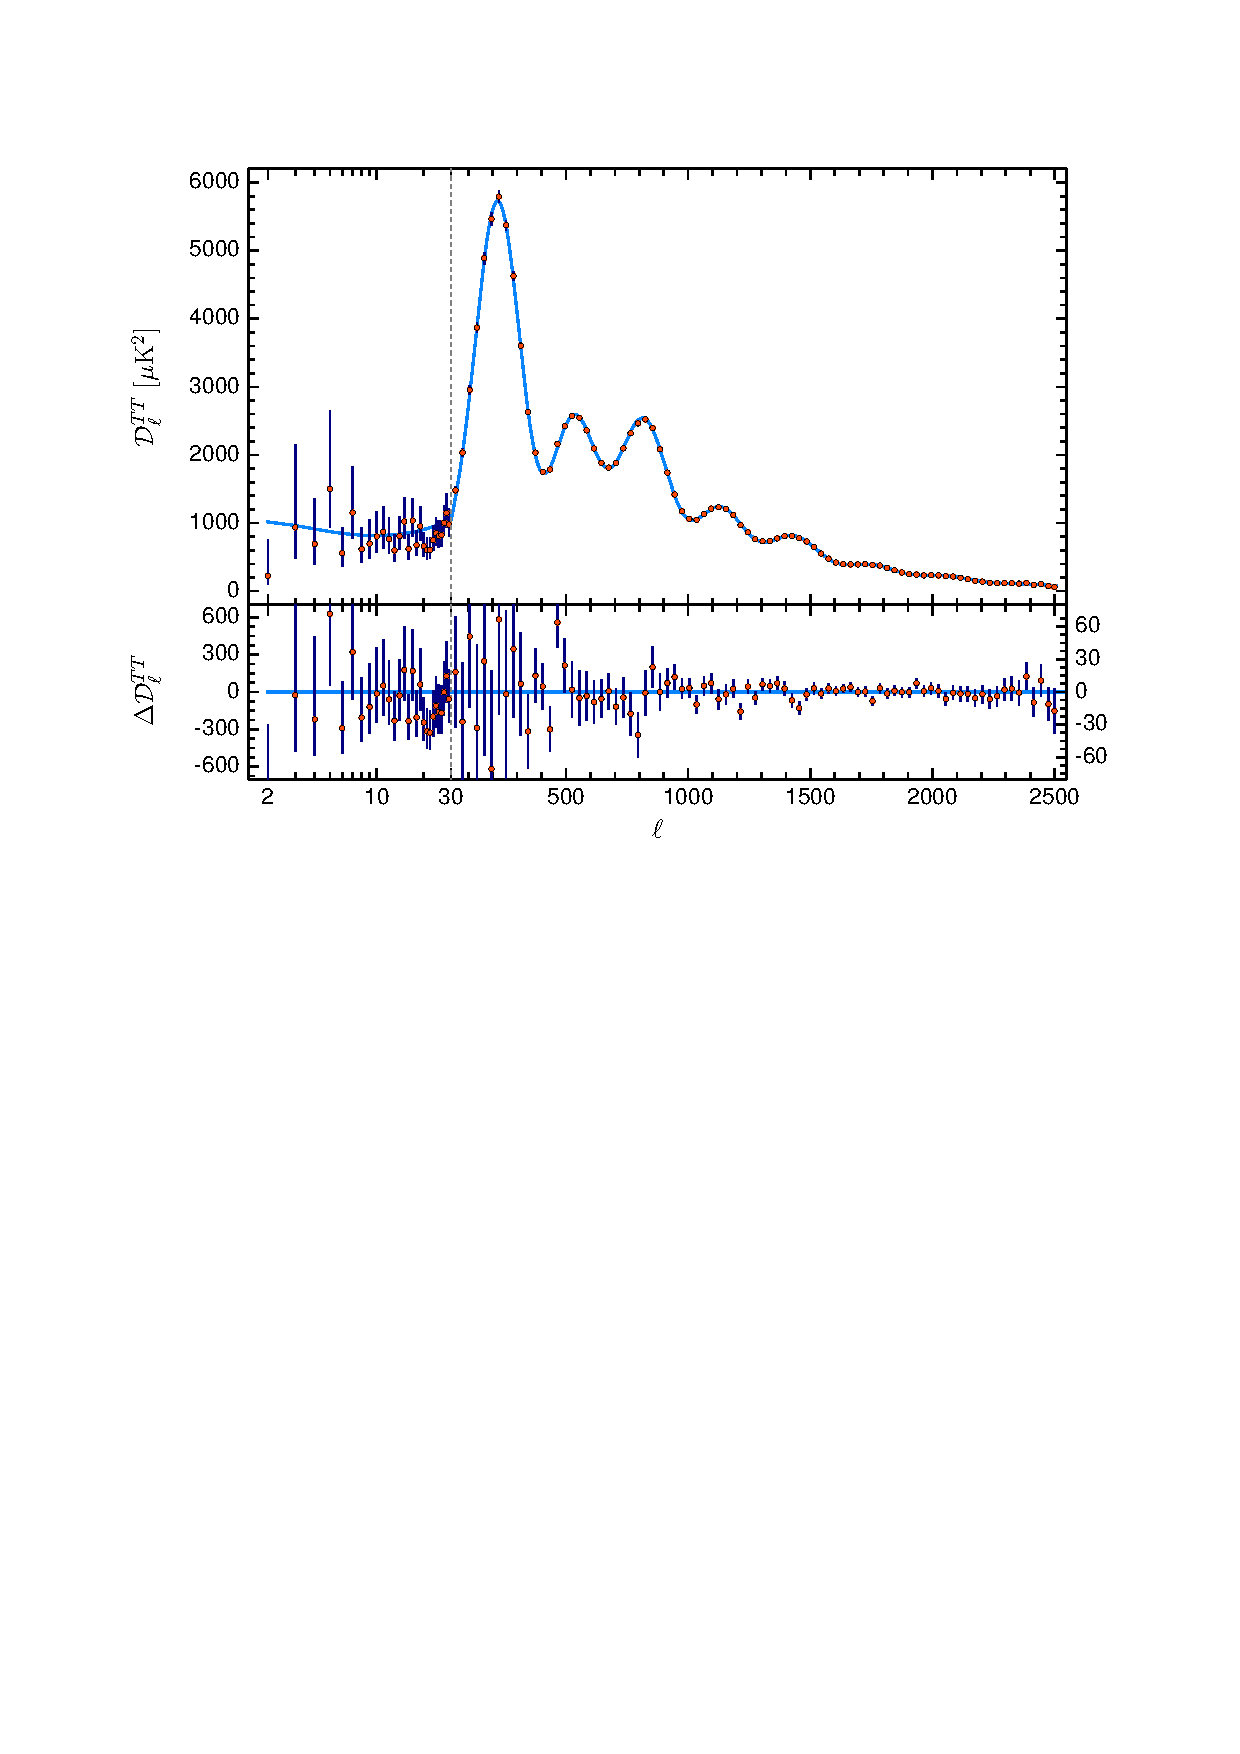
\includegraphics[width=.8\textwidth]{spectrum}
\caption{The (normalized) CMB spectrum. The top panel shows the numerical prediction (from best-fit parameters) in blue and observations in red, while the bottom panel shows the difference between prediction and observation.}
\label{fig:spectrum}
\end{figure}

To see how the temperature anisotropies can be used to infer cosmological parameter we need to understand where the anisotropies come from. Before recombination, in the opaque plasma, the sound speed is 
\begin{align}
c_s = \th{\sqrt{3(1+\frac{3\rho_b}{\rho_\gamma})}},
\end{align}
where $\rho_b$ is the baryon density and $\rho_\gamma$ is the density of photons. Neutrons and dark matter do not affect the sound speed because they are only weakly coupled. In analogy with Eqn.~\ref{eqn:comoving} we can define the comoving sound horizon~\cite{Planck2013}
\begin{align}
r_s(t) = \int_{0}^t \frac{c_s\, dt'}{a}, \label{eqn:rs}
\end{align}
which defines how far density waves can have traveled by  time $t$. 

Since we want to make measurements of the CMB, we care about the sound horizon at last scattering $r_s^*=r_s(t_*)$. Since this value depends only on baryon and photon densities, $r^*_s$ is independent of CMB measurements. From the CMB, we can instead extract the angular scale of the sound horizon at last-scattering, $\theta_s^*$. Unfortunately, there is not a simple formula for $\theta_s^*$. Instead, it is found using the positions of as many peaks in the spectrum as possible. For the \textit{Planck} mission this means seven peaks~\cite{Planck2013, Planck2018}. 

In Euclidean geometry, an object of size $r$ at distance $d>>r$ subtends an angle $\theta = r/d$.
Similarly, the sound horizon and its angular scale are related by
\begin{align}
\theta_s^* = \frac{r_s^*}{D_A^*},
\end{align}
where $D_A$ is the (coming) angular diameter distance.\footnote{Although all sources use the comoving angular diameter distance for this calculation, there is considerable disagreement over what to name the variable. Ref.~\cite{Samtleben2007} uses $d_A$ while Refs.~\cite{Planck2013} and~\cite{DiValentino2021} use $D_A$. Both Ref.~\cite{Planck2018} and Wikipedia~\cite{Wikipedia} use $D_A$ to refer to the proper angular diameter distance, which is equal to the scale factor times the comoving distance.} We can once again appeal to Eqn~\ref{eqn:comoving} to calculate the angular diameter distance as~\cite{Samtleben2007, DiValentino2021}
\begin{align}
D_A^* = \int_{\tau_*}^{\tau_0}d\tau =  \int_0^{z_*}\frac{dz}{H(z)}, \label{eqn:distance}
\end{align}
so that a value of $D_A^*$ can be used to predict $H(z)$. In particular, we can use the CMB pipeline to predict a value of $H(0) = H_0$.

Actually, the whole process is slightly more complicated than that. A more careful analysis shows that the above procedure most directly predicts the reduced density parameters $\omega_b = \Omega_bh^2$ and $\omega_c = \Omega_c h^2$. These predictions can then be combined with local measurements of $\Omega_b$ and $\Omega_c$ to predict the derived parameter $h$ or $H_0$. Ref.~\cite{Planck2018} has nice graphs showing how $h$ and other derived parameter co-vary with the different parameters like $\omega_b$ that are directly predicted by \textit{Planck}. 

Furthermore, the \Planck{} predictions are based not only on the temperature anisotropy spectrum but also on polarization spectra. The gold standard result from \Planck{} uses temperature-temperature, temperature-E-mode, and E-mode-E-mode spectra, plus low-E and lensing data. This pipeline provides a prediction of ${H_0 = \hnaught{67.27 \pm 0.6}}$. Further addition of B-mode polarization and BAO data can further change the prediction, but only slightly.

\subsection{Measurement} \label{sub:measure}

Of course, all that being said, we can follow Hubble's lead and just measure the distance and velocity of objects in our local region. This is complicated by the fact that nearby objects 
have proper motion, meaning that their redshift is not entirely determined by the expansion of the universe. That being said, if we look far enough away we should be able to
see stars or other objects whose motion is dominated by the Hubble flow. These allow us to measure $H_0$ to high accuracy. 

The goal then becomes to find many stars and measure both their velocity and their distance. It is relatively easy to measure velocity using the Doppler effect and the shift in spectrum lines. For nearby stars it is possible to measure distance using parallax. For further distances we rely on types of stars that have very predictable intrinsic luminosities. Then, from the observed velocity, we can infer the distance. The primary types of stars to use are pulsating Cepheid variables and exploding type Ia supernovae~\cite{DiValentino2021}. Together, all these measurements make up the so-called distance ladder.

Cepheid variable stars are stars that pulsate, with a predictable relationship between luminosity and period. This relationship was discovered in 1908 by Henrietta Swan Leavitt~\cite{Leavitt1912} and allows observers to infer the intrinsic luminosity, and thus distance, from period. They are prevalent and bright enough to reach distances of $\SI{10-40}{Mpc}$. Supernovae, while brighter, are much rarer. They are used only to measure velocity at the furthest distances~\cite{DiValentino2021}, and are the last rung on the ladder.

The SH0ES project~\cite{Riess2020} is the current gold standard for observational measurements of the Hubble constant, with a value of $\hnaught{73.2 \pm 1.3}$. Other projects have varying estimates, but they generally agree with the stated value.

\subsection{Summary} \label{sub:sum}

In order to quantify the tension between SH0ES and the \Planck{} measurement, we want to calculate to level of uncertainty the difference between the measurements vanishes~\cite{Dietrich2014}. Explicitly,\footnote{This may be basic statistics, but the author was unable to find the calculation in any of the reference papers, and thought it might be useful to include.} using the values for $h$ to avoid units and letting subscripts distinguish the \Planck{} and SH0ES data, 
\begin{align}
\Delta &= h_1 - h_2 = .6727 - .732 = 5.93,\nn
\sigma &= \sqrt{\sigma_1^2 + \sigma_2^2} = \sqrt{.0060^2 + .013^2} = .0143,\nn
\frac{|\Delta|}{\sigma} &= 4.15,
\end{align}
which is to say that the two measurements disagree at $4.2\sigma$. Other transformations of the data from either the CMB or local measurements can result in slightly different tensions, but they generally lie in the $4\sigma$ to $6\sigma$ range~\cite{DiValentino2021}.

There are other methods of measuring, such as those relying on gravitational waves. Currently, they have high enough uncertainty that they agree with the CMB prediction and the SH0ES observation. If they can significantly decrease uncertainty they may come out of agreement with one or the other. New methods
will not relieve tension if they agree with observations, but can say whether or not SH0ES data has  systematics.
Fig.~\ref{fig:whisker} shows the value and uncertainty of $H_0$ using many different methods. 

\begin{figure}
\centering
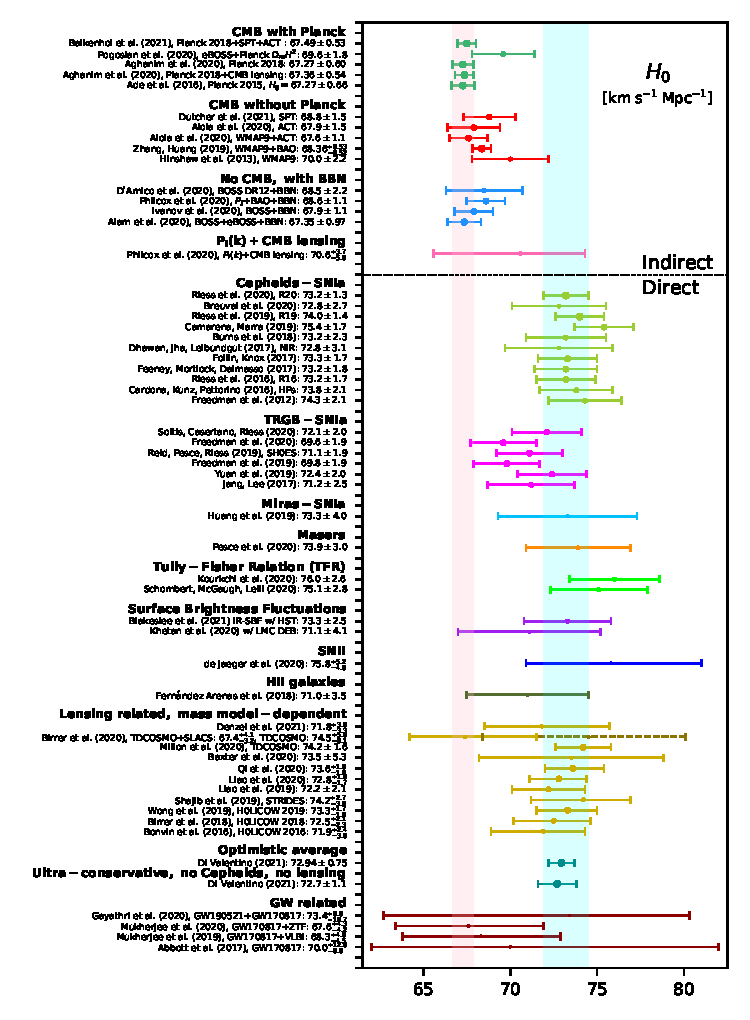
\includegraphics[width=.91\textwidth]{whisker}
\caption{A summary of many different indirect and direct measurements of the Hubble constant, taken from Ref.~\cite{DiValentino2021}. The values quoted in the current paper are the third from the top and the first in the ``indirect" section. This figure is included to show that there are many methods in addition to those described in the current paper for measuring $H_0$. Direct measurements in general favor a higher value, although sometimes with very large error bars.}
\label{fig:whisker}
\end{figure}

\section{Possible resolutions} \label{sec:resol}

The simplest possible resolution to the Hubble tension would be that we are still not measuring velocities far enough out in the universe, so that our local value of $H_0$ is not the correct value for our entire timeslice. This possibility is highly unlikely. It would require that our local Universe is about 20 times more underdense than statistical fluctuations suggest is likely~\cite{DiValentino2021}. There are many more proposed ways to resolve the Hubble tension. In this section we will review a few methods that invoke modified dark energy, followed by a quick rundown of alternative methods.

\subsection{Modified dark energy} \label{sub:dark}

In some sense, the most phenomenological element of the \L CDM model is dark energy. If we claim that $\rho_\Lambda$ is equal to the vacuum energy of the effective field theory of the Standard Model, it is off by a stunning 120 orders of magnitude~\cite{Trodden2004}. Thus, it is tempting to modify its contribution to the Friedmann equations before any other component.
The first type of modification we will consider is Early Dark Energy (EDE, \val{4}). These models have an extra flavor of dark energy that existed at early times but does not exist now. This changes evolution in the pre-reionization plasma, decreasing $r_s$. 

Our first example of EDE is a scalar field $\phi$ performing sitting in an anharmonic potential, ${V(\phi) = [1-\cos(\phi/f)]^n}$. The scalar field sits still at the bottom of the potential until a critical time $t_c$ when it begins to oscillate. Its equation of state as a function of $a$ is
\begin{align}
w_\phi(a) = -1 + \frac{1+w_n}{1+ (a_c/a)^{3(1+w_n)}},
\end{align}
where $w_n = (n-1)/(n+1)$ and $a_c = a(t_c)$ is the scale factor at the critical time. Thus, at early times $phi$ behaves like a cosmological constant with $w_\phi\approx -1$ and at late times it has an effective equation of state $w_\phi=w_n$. This would correspond to matter for $n=1$ and radiation for $n=2$, while for $n=3$ it can help decrease the Hubble tension to $2\sigma$.

A popular fad in the world of EDE is Rock `n' Roll, which is also a model of a scalar field $\phi$. Now, the field lives in a potential
\begin{align}
V(\phi) = V_0\left(\frac{\phi}{M_\text{Pl}}\right)^{2n} + V_1,
\end{align}
where $V_0$ and $V_1$ are constants, $n$ is an index, and $M_\text{Pl} = (8\pi G)^{-1/2}$ is the Planck mass. Once this field begins to oscillate, it either oscillates for all time (rocking), or asymptotes to a rolling solution. Models from this class claim to resolve the tension to $1.9\sigma$, but more careful analysis shows they only decrease it to $3.3\sigma$.

Late dark energy (LDE, \val{5}) instead changes the equation of state for the component of dark energy that we do see. A different equation of state for dark energy changes the angular diameter distance (Eqn.~\ref{eqn:distance}) by modifying the first Friedman equation (Eqns.~\ref{eqn:fri1} and~\ref{eqn:pevolve}). The simplest LDE model is the $w$CDM model, where dark energy has a constant equation of state $w_\DE\ne-1$. A $w$CDM model can completely alleviate the Hubble tension, at the cost of introducing phantom-like dark energy, $w_\DE<-1$. From Eqn.~\ref{eqn:pevolve} we can see that such a flavor of dark energy would have an energy density that increases with time. Then the first Friedmann equation tells us that the scale factor $a$ will diverge in finite time, a situation called the Big Rip.

%Many other LDE models allow the dark energy equation of state to vary with $a$. These equations of state generically depend on the current value $w_0$ (need not be $-1$) and another parameter $w_a$ that describes the evolution. For example the CPL parameterization $w_\DE(a) = w_0 + (1-a)w_a$ allows $w_\DE$ to change from $w_0+w_a$ at the beginning of the Universe to $w_0$ now. Ref.~\cite{DiValentino2021} lists many other possible parameterizations with either one or two free parameters. 

EDE and LDE models all alleviate the Hubble tension in part by increasing the number of free parameters compared to the \L CDM model. Since all these models are phenomenological anyway, we should try to match the number of parameters in \L CDM. This class of models with six degrees of freedom (\val{6}) includes Phenomenologically Emergent Dark Energy (PEDE). The equation of state is
\begin{align}
w_\text{PEDE} = -1 -\th{3\ln 10} [1 + \tanh \log_{10}(1 + z)],
\end{align}
and the model can resolve the Hubble tension to within $1\sigma$.

\subsection{Other possible resolutions} \label{sub:other}

There are many other possible resolutions to the Hubble tension. Here we will very briefly review a handful of categories of theories from Ref.~\cite{DiValentino2021} before concluding. Recall that the ingredients of the \L CDM model are General Relativity with the FLRW metric, some form of dark energy \L, cold dark matter, the Standard Model of matter we can see, and a history of the Universe. Since we already focused on theories that modify dark energy, the remaining theories will change some other ingredient.

The first class contains theories with extra relativistic degrees of freedom (\val{7}), in the form of a higher effective number of neutrinos, $N_\eff$. This shifts the peaks in the CMB by increasing $\rho_r$ and $\Omega_r$. Alternatively, we can consider extra interactions between dark energy and dark matter or between either of the two dark fluids and ordinary matter (\val{8}). These allow the different forms of energy density and pressure to interconvert, modifying Eqn.~\ref{eqn:pevolve}. 

A fun example of an extra interaction model is the $L_\mu-L_\tau$ model~\cite{Escudero2019}, which includes a massive $Z'$ boson that decays into neutrinos. The authors claim that this form of extension to the Standard Model, while largely unconstrained, is able to solve both the Hubble tension and the longstanding and recently-confirmed tension in measurements of the muon magnetic moment~\cite{Muon2021}.

The interaction models are taken to the extreme in so-called unified dark fluid models (\val{9}). In these theories, there is a single dark fluid, with a time-dependent equation of state, that behaves like dark matter in the early Universe and dark energy in the late Universe. 

Finally, there are theories of modified gravity, inflation, modified behavior at recombination, phase transitions in dark energy, and other possibilities (\val{10-14}). At the time of the publication of Ref.~\cite{DiValentino2021} many of these models had not been analyzed using the most recent \textit{Planck} 2018 data, so reanalysis might be useful. For all of these models, the quantitative reduction in tension can be found in Fef.~\cite{DiValentino2021}.

\section{Conclusion} \label{sec:concl}

\outline{lensing, polarization, BAO}

\outline{Testing ground for new physics}

\bibliographystyle{unsrt}
\bibliography{hubbletension}

\end{document}